\documentclass[10pt,a4paper]{article}
\usepackage[utf8]{inputenc}
\usepackage[danish]{babel}
\usepackage{amsmath}
\usepackage{amsfonts}
\usepackage{amssymb}
\usepackage{graphicx}
\usepackage[left=2cm,right=2cm,top=2cm,bottom=2cm]{geometry}


\usepackage{titlepic}
\usepackage{enumerate}
\usepackage{enumitem}
\usepackage{float}
\usepackage{pdfpages}
\usepackage[colorlinks = true,
            linkcolor = blue,
            urlcolor  = blue,
            citecolor = blue,
            anchorcolor = blue]{hyperref}
\usepackage[explicit]{titlesec}
\usepackage{pstricks}
\usepackage[amsmath,thmmarks]{ntheorem} %pakke til at lave sætningsenvorinmets (kan ikke loades sammen med amsthm)
\usepackage{color}
\usepackage{tikz}

%opretter environmets til sætningsstrukturen 
\theorembodyfont{\normalfont}

	
	%sætnings environment	
	\newtheorem{thm}{Sætning}

	\theoremstyle{break}	
	%opgave environment	
	\newtheorem{opg}{Opgave}	

	%Korrolar environment
	\newtheorem{korollar}[thm]{Korollar}	
	
	%Lemma environment	
	\newtheorem{lemma}[thm]{Lemma}
	
	\theoremsymbol{\ensuremath{\circ}}	
	
	%definition environment	
	\newtheorem{definition}[thm]{Definition}
	
	%eksempel environment	
	\newtheorem{eksempel}[thm]{Eksempel}
	
	
	
	%Bevis environment
	\theoremstyle{nonumberplain}
	\theoremheaderfont{%
	\normalfont\itshape}
	\theorembodyfont{\normalfont}
	\theoremsymbol{\ensuremath{\square}}
	\theoremseparator{.}
	
	\newtheorem{proof}{Bevis}
	\newtheorem{los}{Løsning}
	






\setlength\parindent{0pt}

%\titleformat{\section}{\Large\bfseries}{}{0pt}{#1}
%\titleformat{\subsection}{\large\bfseries}{}{0pt}{#1}


%nye komandoer
\newcommand{\mR}{\mathbb{R}}
\newcommand{\mZ}{\mathbb{Z}}
\newcommand{\mN}{\mathbb{N}}
\newcommand{\mQ}{\mathbb{Q}}
\newcommand{\mC}{\mathbb{C}}
\newcommand{\hs}{\hspace{2mm}}
\newcommand{\Hs}{\hspace{4mm}}
\newcommand{\pipe}{\hs | \hs}
\newcommand{\lp}{\left(}
\newcommand{\rp}{\right)}
\newcommand{\vect}[1]{\underline{#1}}
\newcommand{\matr}[1]{\underline{\underline{#1}}}
\newcommand{\cnum}[1]{\raisebox{.5pt}{\textcircled{\raisebox{-.9pt} {#1}}}}




\author{Mikkel B. Goldschmidt\\3r, Nørre Gymnasium}
\title{Laplace lov}
\date{\today}



\begin{document}
\maketitle

\section{Indledning}
Laplaces lov beskriver den kraft, F, der påvirker en elektrisk leder leder med længde, l, hvorigennem der løber en strøm med styrke I, der er anbragt i et magnetfelt med styrke, B, med en vinkel $\Theta$ mellem magnetfeltet og lederen.

Den siger at: 
$$F=B \cdot I \cdot L\cdot \sin (\theta)$$

\section{Teori}
Her skal der stå noget teori... tjek bogen.

\section{Forsøgsbeskrivelse}
Vi udførte tre forsøg til at bekræfte loven. 
I alle tre forsøg har vi haft en ''Hestesko''-magnet anbragt på en vægt. 
Ned imellem de to poler nede i hesteskoen, satte vi en elektrisk fastsat på en plade der var sat i et stativ.
Gennem denne leder løb der jævnstrøm, der kunne justeres fra en strømforsyning. 
I serieforbindelse mellem strømforsyningen og og lederen var et amperemeter placeret.
På figur \ref{opstilling} kan ses et billede af den beskrevne opstilling.	


\begin{figure}[h]
\center
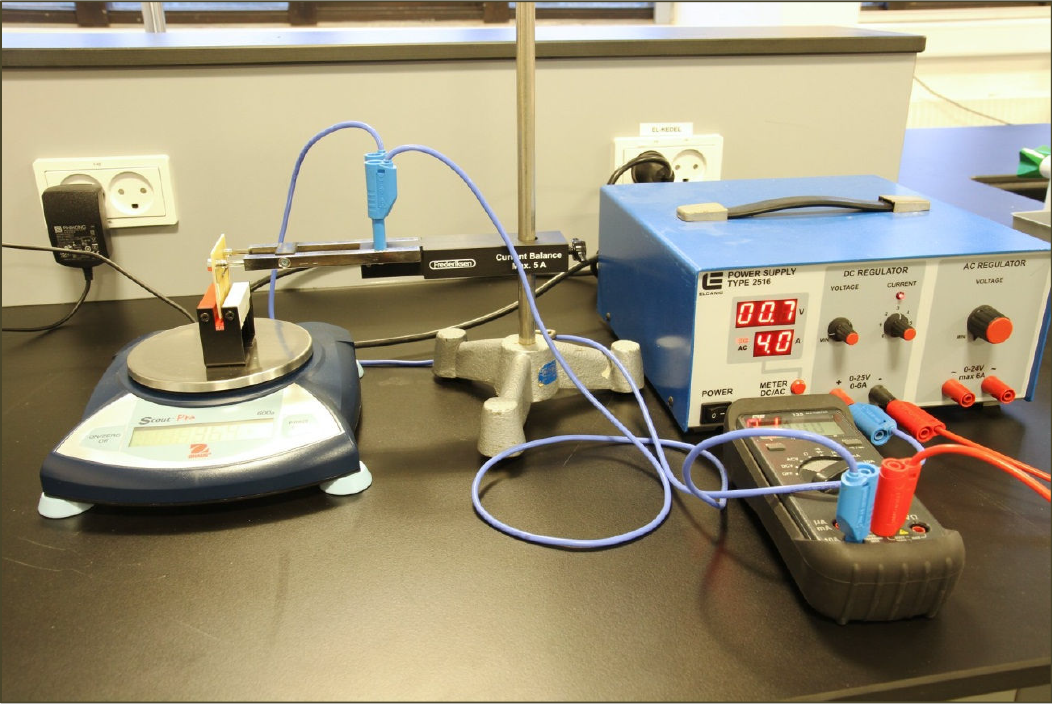
\includegraphics[scale=0.4]{opstilling}
\caption{Et billede af forsøgsopstillingen for alle tre delforsøg. Billedet er taget af Erik Westergaard fra www.matematikogfysik.dk}
\label{opstilling}
\end{figure}

Vi lavede da tre måleserier hvor vi kiggede på ændringen i $F$, nå vi varierede henholdsvist $B,I$ og $L$, mens vi holdt de andre konstante. 




\end{document}